
\definecolor{blueLine}{RGB}{57,106,177}
\definecolor{blueFill}{RGB}{114,147,203}
\definecolor{redLine}{RGB}{204,37,41}

\begin{figure}[t]
\centering
% \vspace{-0.1in}
%    \makebox[\linewidth]{
       % 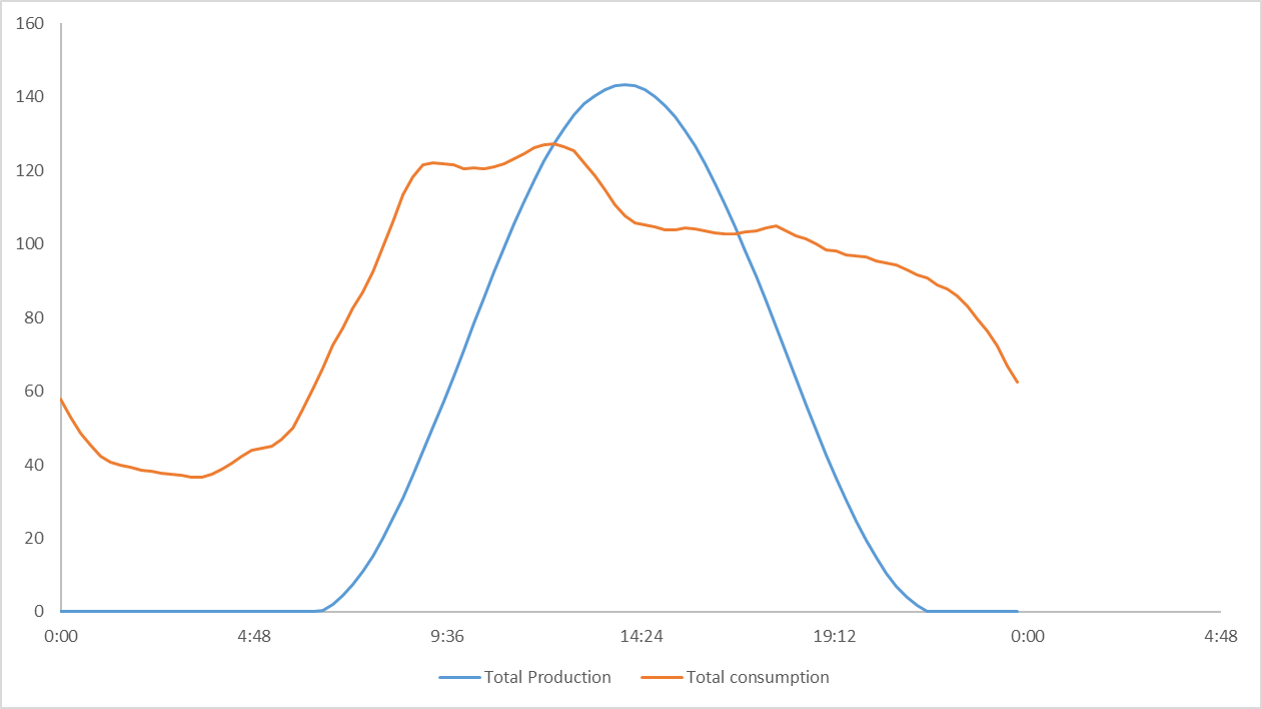
\includegraphics[width=1.0\linewidth]{loadprofile.png}
%    }

\begin{tikzpicture}
\begin{axis}[
  font=\small,
  width=1.05\columnwidth,
  height=0.61\columnwidth,
  ymin=-1,
  ymax=200,
  xmin=-1,
  xmax=97,
  legend pos=north west,
  xlabel=Time,
  ylabel={[kWh]},
  ytick={0, 50, 100, 150},
  xtick={0, 32, 64, 95},
  xticklabels={0:00, 8:00, 16:00,  23:45},
%  ymajorgrids,
%  xmajorgrids,
]
\addplot[no markers, solid, blueLine, semithick] table[x expr=\coordindex, y=Production, comment chars={\%}] {total_prod_cons.csv};
\addlegendentry{Total production};
\addplot[no markers, solid, redLine, semithick] table[x expr=\coordindex, y=Consumption, comment chars={\%}] {total_prod_cons.csv};
\addlegendentry{Total consumption};
\end{axis}
\end{tikzpicture}
\vspace{-2em}
\caption{Load profile and Generation Profile in KWH per 15 minute interval. The horizontal axis shows time of day.}
\label{fig:profile}
% \vspace{-0.2in}
\end{figure}

We use  data collected by Siemens, from a microgrid in Germany,  to demonstrate a simulated transactive scenario. Figure \ref{fig:profile} shows the total energy produced in this system over the day, and  the total energy consumed. We use a $T=15$ minute time interval for bids and asks. We picked a 3.5 hour time interval (from 2:15pm to 5:45pm) and 2 producers and 7 consumers that overlapped with the peak of production capacity (see Figure \ref{fig:profile}). We ran the network across six virtual machines, each with 2 virtual CPUs, 4 GB RAM and 40 GB hard-disk. The \texttt{geth} clients (one per actor) and miners were equally distributed on this network. The actors (Prosumers and DSO) were written in Python, and they communicated with the \texttt{geth} clients using JSON-RPC API provided by Ethereum. The  actors communicated with each other using RIAPS and polled the blockchain ledger for transactional updates using custom filters, which are supported by the Ethereum API.
%\Aron{We could claim that we picked this time interval because it was the busiest.}}} The system has $2$  producers and 7 consumers from a microgrid installation in Germany.  
%\Abhishek{Mike - please explain the figures. they both look very similar.}

Figure~\ref{fig:offer_histogram} shows the distribution of the time between when an offer was made by a producer, and then the time when the offer was accepted by a consumer and cleared. As shown by Figure~\ref{fig:workflow}, this includes two transactions, \texttt{postOffer} and \texttt{acceptOffer}, which have to be verified and recorded by the miners. To clear these two transactions, at least two blocks need to be mined. The statistics of the clearing-time distribution are as follows: 
average = 11.79 seconds, median = 11 seconds, variance = 46.74, maximum = 38 seconds, minimum = 0 seconds, and 90\% of trades were cleared within 23 seconds or less.

%Figure \ref{} shows the setup of virtual machines on which we play out the simulated transactions capturing the timing restrictions and showing the feasibility of the system, while maintaining the safety constraints and the privacy restrictions. 


\begin{figure}[t]
% \vspace{-0.1in}
%    \makebox[\linewidth]{
       % 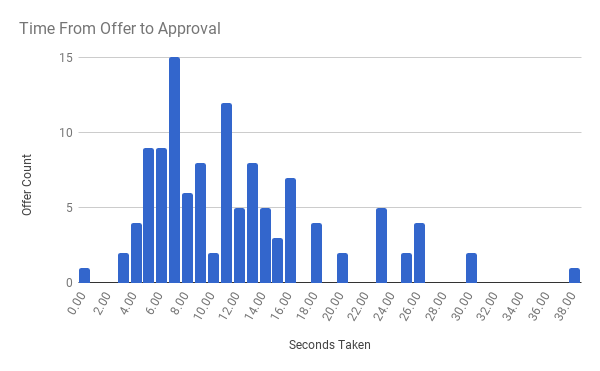
\includegraphics[width=1.0\linewidth]{offer_histogram.png}
%        }
  \begin{tikzpicture}
\begin{axis}[
  font=\small,
  width=1.05\columnwidth,
  height=0.54\columnwidth,
  ymin=0,
  ymax=16,
  xmin=-0.5,
  xmax=38.5,
  xlabel={Time until offer was accepted [seconds]},
  ylabel={Number of offers},
  ymajorgrids,
]
\addplot[ybar, bar width=3pt, no markers, fill=blueFill, draw=blueLine, semithick] table[x=Seconds, y=Count, comment chars={\%}, col sep=comma] {TimePerOfferHistogram.csv};
\end{axis}
\end{tikzpicture}
\vspace{-1em}
\caption{Histogram of time it takes to clear the two transactions related to post offer and accept offer. 90\% of the trades were closed within 23 seconds or less.}
\label{fig:offer_histogram}
% \vspace{-0.2in}
\end{figure}

